\documentclass{article}
\usepackage{float}
\usepackage{amsmath}
\usepackage{graphicx}
\usepackage{hyperref}
\usepackage{geometry}
\usepackage{amsfonts}
\usepackage{amssymb}
\usepackage{algorithm}
\usepackage{algorithmic}
\usepackage{graphicx}
\usepackage{multirow}
\usepackage{multicol}
\usepackage{subcaption}

\DeclareMathOperator*{\argmax}{arg\,max}
\DeclareMathOperator*{\argmin}{arg\,min}
% \geometry{a4paper, margin=1in}
\usepackage[sorting=none]{biblatex}
\addbibresource{bibliography.bib}

\usepackage{color}
\definecolor{darkred}{rgb}{0.6,0.0,0.0}
\definecolor{darkgreen}{rgb}{0,0.50,0}
\definecolor{lightblue}{rgb}{0.0,0.42,0.91}
\definecolor{orange}{rgb}{0.99,0.48,0.13}
\definecolor{grass}{rgb}{0.18,0.80,0.18}
\definecolor{pink}{rgb}{0.97,0.15,0.45}

% listings
\usepackage{listings}

% General Setting of listings
\lstset{
  aboveskip=1em,
  breaklines=true,
  abovecaptionskip=-6pt,
  captionpos=b,
  escapeinside={\%*}{*)},
  frame=single,
  numbers=left,
  numbersep=15pt,
  numberstyle=\tiny,
}
% 0. Basic Color Theme
\lstdefinestyle{colored}{ %
  basicstyle=\ttfamily,
  backgroundcolor=\color{white},
  commentstyle=\color{green}\itshape,
  keywordstyle=\color{blue}\bfseries\itshape,
  stringstyle=\color{red},
}
% 1. General Python Keywords List
\lstdefinelanguage{PythonPlus}[]{Python}{
  morekeywords=[1]{,as,assert,nonlocal,with,yield,self,True,False,None,} % Python builtin
  morekeywords=[2]{,__init__,__add__,__mul__,__div__,__sub__,__call__,__getitem__,__setitem__,__eq__,__ne__,__nonzero__,__rmul__,__radd__,__repr__,__str__,__get__,__truediv__,__pow__,__name__,__future__,__all__,}, % magic methods
  morekeywords=[3]{,object,type,isinstance,copy,deepcopy,zip,enumerate,reversed,list,set,len,dict,tuple,range,xrange,append,execfile,real,imag,reduce,str,repr,}, % common functions
  morekeywords=[4]{,Exception,NameError,IndexError,SyntaxError,TypeError,ValueError,OverflowError,ZeroDivisionError,}, % errors
  morekeywords=[5]{,ode,fsolve,sqrt,exp,sin,cos,arctan,arctan2,arccos,pi, array,norm,solve,dot,arange,isscalar,max,sum,flatten,shape,reshape,find,any,all,abs,plot,linspace,legend,quad,polyval,polyfit,hstack,concatenate,vstack,column_stack,empty,zeros,ones,rand,vander,grid,pcolor,eig,eigs,eigvals,svd,qr,tan,det,logspace,roll,min,mean,cumsum,cumprod,diff,vectorize,lstsq,cla,eye,xlabel,ylabel,squeeze,}, % numpy / math
}
% 2. New Language based on Python
\lstdefinelanguage{PyBrIM}[]{PythonPlus}{
  emph={d,E,a,Fc28,Fy,Fu,D,des,supplier,Material,Rectangle,PyElmt},
}
% 3. Extended theme
\lstdefinestyle{colorEX}{
  basicstyle=\ttfamily,
  backgroundcolor=\color{white},
  commentstyle=\color{darkgreen}\slshape,
  keywordstyle=\color{blue}\bfseries\itshape,
  keywordstyle=[2]\color{blue}\bfseries,
  keywordstyle=[3]\color{grass},
  keywordstyle=[4]\color{red},
  keywordstyle=[5]\color{orange},
  stringstyle=\color{darkred},
  emphstyle=\color{pink}\underbar,
}


\title{Using LDA for Topic Modeling on Song Lyrics}
\author{Chenye Yang, Hanchu Zhou, Haodong Liang, Yibo Ma}
\date{June 13, 2024}

\begin{document}

\maketitle

\section{Introduction}\label{sec:introduction}

Analyzing the thematic content of song lyrics presents a fascinating and challenging problem in the field of natural language processing (NLP). Song lyrics can be regarded as a unique form of text that often convey deep emotions and complex narratives within a highly structured and sometimes repetitive linguistic framework. Unlike more straightforward text data, lyrics can feature abstract metaphors, colloquial language, and varying levels of ambiguity, all of which are set to rhythm and melody that influence their interpretation. Such analysis can benefit a range of applications, from enhancing music recommendation systems to aiding in the study of cultural and societal trends through music.\\

\noindent Topic modeling has been widely used in various fields to uncover hidden structures in text data. Blei et al. (2003) introduced latent Dirichlet allocation (LDA)~\cite{blei2003latent}, which is a generative probabilistic model that allows sets of text elements to be explained by unobserved groups, providing a way to uncover the hidden thematic structure in a large collection of texts. LDA has since become a standard technique for discovering topics in large corpora. Previous studies have applied LDA to analyze scientific publications, news articles, and social media posts. The potential of LDA to analyze song lyrics, however, remains relatively unexplored. \\

\noindent While LDA is adept at modeling textual data, Dictionary Learning~\cite{olshausen1996emergence, arora2018linear} works as a complementary technique, particularly effective in fields requiring robust feature extraction such as image and signal processing. This method involves decomposing a dataset into a dictionary of basis functions and sparse representations, where each data element is expressed as a sparse linear combination of these basis atoms. The focus in Dictionary Learning is on reconstructing the input data with high fidelity, employing a minimal number of active dictionary elements to achieve efficient and compact data representations. The choice of LDA and Dictionary Learning depends on the nature of the data and the analytical goals, whether it is uncovering thematic patterns in text with LDA or achieving sparse and efficient representations in multimedia data with Dictionary Learning.\\

\noindent In addition to LDA, the Term Frequency-Inverse Document Frequency (TF-IDF)~\cite{sparck1972statistical} model is another crucial technique in the landscape of text analysis. Unlike LDA, which focuses on discovering latent topics, TF-IDF is a statistical measure used to evaluate how important a word is to a document in a collection or corpus. It is often employed as a weighting factor in searches of information retrieval, text mining, and user modeling. The importance increases proportionally to the number of times a word appears in the document but is offset by the frequency of the word in the corpus, which helps to adjust for the fact that some words appear more frequently in general.\\

\noindent TF-IDF can be particularly effective in distinguishing the relevance of words in large datasets and has been applied extensively in document classification and clustering, spam filtering, and even in sentiment analysis. Its ability to transform the textual data into a numeric form and assess word relevance through both local and global document contexts makes it a valuable complement to LDA in comprehensive text analysis strategies. The combined use of LDA for topic discovery and TF-IDF for importance weighting could potentially provide deeper insights into the thematic elements of song lyrics, enhancing our understanding of linguistic patterns and cultural influences reflected in music.\\

\noindent In this project, we aim to discover the underlying topics in a dataset of song lyrics using TF-IDF and LDA. The goal is to categorize the lyrics into distinct themes and analyze the distribution of these themes across different songs and artists. We preprocess the lyrics, vectorize them using TF-IDF, and fit the LDA model to identify the topics. The results provide insights into the thematic content of the song lyrics and can be used for further analysis or applications in music recommendation systems.



\section{Data Collection}

The dataset was compiled using the Genius API~\cite{geniusapi}, which provides access to a vast collection of song lyrics. We selected a diverse range of artists and genres to ensure a representative sample. The dataset includes lyrics from well-known artists in Hip Hop, Country, Pop, Rock, Jazz, and Classic. The lyrics were preprocessed to remove non-English words, stopwords, and special characters, ensuring that only valid English words were included in the analysis. The resulting dataset contains a collection of singers, albums, and song lyrics ready for vectorization and topic modeling, shown in Figure~\ref{fig:lyrics}.

\begin{figure}[H]
    \centering
    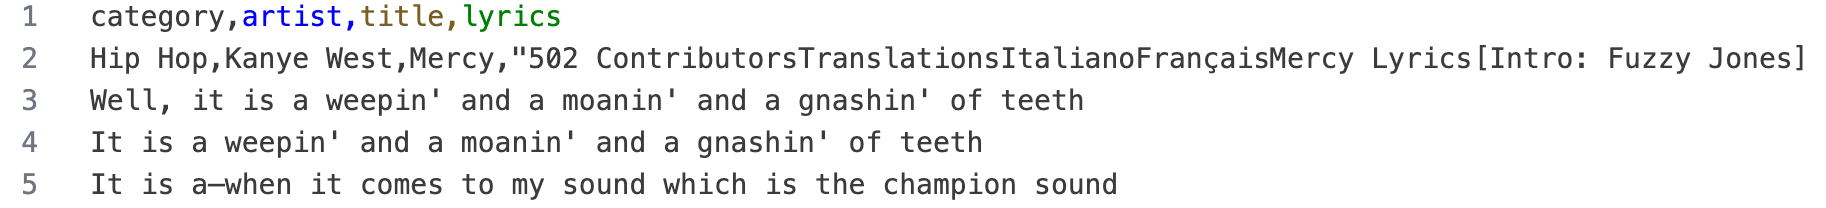
\includegraphics[width=\textwidth]{lyrics.png}
    \caption{Example of Lyrics Dataset}
    \label{fig:lyrics}
\end{figure}

\section{Method}

\subsection{Word Vectorization}

Word Vectorization is a crucial step in preparing the lyrics for analysis. The following steps were performed:

\subsubsection{Lyrics Preprocessing}
\begin{enumerate}
    \item[i.] \textbf{Tokenization}: Splitting the lyrics into individual words.
    \item[ii.] \textbf{Stopwords Removal}: Removing common words that do not contribute much to the meaning (e.g., "the", "is", "and").
    \item[iii.] \textbf{Custom Stopwords}: Additional stopwords specific to song lyrics (e.g., "chorus", "yeah", "ooh").
    \item[iv.] \textbf{Filtering Non-English Words}: Ensuring only valid English words are considered.
    \item[v.] \textbf{Normalization}: Converting all words to lowercase and removing non-alphabetic characters.
\end{enumerate}

\subsubsection{TF-IDF Embedding}
We use tf-idf vectorization to convert the preprocessed lyrics into numerical vectors. This is a common transformation used in text analysis to represent the importance of a word in a document relative to a collection of documents. The transformation is given by the following steps:
\begin{enumerate}
    \item [i.] \textbf{Term Frequency (TF)}: Count the number of times word $t$ appears in document $d$, denoted as \[TF(t,d)=f_{t,d}\]
    \item [ii.] \textbf{Inverse Document Frequency (IDF)}: Calculate the inverse document frequency of word $t$ in the entire corpus, denoted as \[IDF(t)=\log\left(\frac{N}{df_t}\right)\]
    where $N$ is the total number of documents and $df_t$ is the number of documents containing word $t$.
    \item [iii.] \textbf{TF-IDF}: The TF-IDF value of word $t$ in document $d$ is given by \[TFIDF(t,d)=TF(t,d)\times IDF(t)\]
\end{enumerate}

\noindent In general, the TF-IDF value increases with the number of times a word appears in a document but is offset by the frequency of the word in the entire corpus, making it highlight the distinctive words that are frequently appeared in a document but not common in the entire corpus.

\subsection{Latent Dirichlet Allocation}
\subsubsection{Model Overview}
Latent Dirichlet Allocation (LDA) is a two-layer hierarchical Bayesian model that represents documents as random mixtures of latent topics. Each topic is characterized by a distribution over words. The structure of LDA model is shown in Figure ~\ref{fig:lda}. 


\begin{figure}[H]
    \centering
    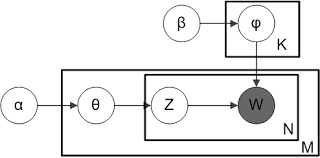
\includegraphics[width=0.5\textwidth]{lda.png}
    \caption{Latent Dirichlet Allocation (LDA) Model}
    \label{fig:lda}
\end{figure}

\noindent In the above figure, $\alpha$ and $\beta$ are hyperparameters of Dirichlet Distribution, $N$ is the number of words in a document, $K$ is the number of topics, $M$ is the number of documents, $z$ is the topic assignment for each word, and $w$ is the word. \\

\noindent The LDA model assumes the following generative process for each document $d$:
\begin{enumerate}
    \item Draw $\theta_d \sim \text{Dir}(\alpha)$ for each document $d$
    \item Draw $\phi_k \sim \text{Dir}(\beta)$ for each topic $k$
    \item For each word $w_{d,n}$ in document $d$:
    \begin{enumerate}
        \item Choose a topic $z_{d,n} \sim \text{Multinomial}(\theta_d)$
        \item Choose a word $w_{d,n} \sim \text{Multinomial}(\phi_{z_{d,n}})$
    \end{enumerate}
\end{enumerate}

\subsubsection{Variational Inference}
\noindent Estimating the parameters of the Latent Dirichlet Allocation (LDA) model involves inferring the posterior distribution of the latent variables given the observed data. Since exact inference is intractable, approximate methods are used. One of the common approaches for parameter estimation in LDA is Variational Inference.\\

\noindent We approximate the posterior distribution $p(\theta,\phi,z|w,\alpha,b)$ with a variational distribution $q(\theta,\phi,z|\gamma,\lambda,\psi)$: \[q(\theta,\phi,z|\gamma,\lambda,\psi)=q(\theta|\gamma)q(\phi|\lambda)\prod_{d=1}^M\prod_{n=1}^{N_d}q(z_{d,n}|\psi_{d,n})\]
where $q(\theta|\gamma)$ is the variational distribution of $\theta_d$, $q(\phi|\lambda)$ is the variational distribution of $\phi_k$, $q(z_{d,n}|\psi_{d,n})$ is the variational distribution of $z_{d,n}$. We assume independence between the latent variables so that the joint distribution can be factorized.\\

\noindent We want to minimize the KL divergence:
\begin{equation*}
    \begin{split}
\argmin_{\gamma,\lambda,\phi}KL(q(\theta,\phi,z|\gamma,\lambda,\psi)||p(\theta,\phi,z|w,\alpha,\beta))&=\mathbb{E}_q[\log q(\theta,\phi,z)]-\mathbb{E}_q[\log p(\theta,\phi,z|w)]\\
        &=\mathbb{E}_q[\log q(\theta,\phi,z)]-\mathbb{E}_q[\log p(w,\theta,\phi,z)]+\log p(w)
    \end{split}
\end{equation*}\\

\noindent We know that minimizing the KL divergence is equivalent to maximizing the Evidence Lower Bound (ELBO). Then we can derive ELBO as the objective function for optimization:
\begin{equation*}
    \begin{split}
        \mathcal{L}(q)&=\mathbb{E}_q[\log p(w,z,\theta,\phi|\alpha,\beta)]-\mathbb{E}_q[\log q(\theta,\phi,z)]\\
        &=\mathbb{E}_q[\log p(w|\phi,z)]+\mathbb{E}_q[\log p(z|\theta)]+\mathbb{E}_q[\log p(\theta|\alpha)]+\mathbb{E}_q[\log p(\phi|\beta)]\\&\quad-\mathbb{E}_q[\log q(\theta)]-\mathbb{E}_q[\log q(\phi)]-\mathbb{E}_q[\log q(z)]
    \end{split}
\end{equation*}\\

\noindent To optimize the ELBO, we iteratively update the variational parameters $\gamma$, $\lambda$, and $\psi$ until convergence. Note that Dirichlet distribution is the conjugate prior of the multinomial distribution, so we can derive the optimization steps are as follows:
\begin{enumerate}
    \item[i.] Update $\psi$: \[
        \psi_{dnk} \propto \beta_{kw_{dn}} \exp\left( \mathbb{E}_{q}[\log \theta_{dk}] \right)
        \]
    \item[ii.] Update $\gamma$:  \[
        \gamma_{dk} = \alpha_k + \sum_{n=1}^{N_d} \psi_{dnk}
        \]
    \item[iii.] Expectation of Log Topic Proportions:
        \[
        \mathbb{E}_{q}[\log \theta_{dk}] = \Psi(\gamma_{dk}) - \Psi\left( \sum_{j=1}^{K} \gamma_{dj} \right)
    \]
    \noindent where $\Psi(\cdot)$ is the digamma function.
    \item[iv.] Update $\lambda_{k,v}$:
        \[
        \lambda_{kv} = \beta_{v} + \sum_{d=1}^{M} \sum_{n=1}^{N_d} \psi_{dnk} \mathbb{I}(w_{dn}=v)
        \]
    \item[v.] Expectation of Log Word Distributions:
        \[
        \mathbb{E}_{q}[\log \phi_{dk}] = \Psi(\lambda_{kv}) - \Psi\left( \sum_{j=1}^{V} \lambda_{kj} \right)\]
\end{enumerate}

\noindent The algorithm is summarized in Algorithm~\ref{algo:lda}.
\begin{algorithm}
\caption{Variational Inference for LDA}
\begin{algorithmic}[1]\label{algo:lda}
\STATE Initialize $\gamma,\lambda$ and $\psi$ randomly.
\REPEAT
    \FOR{each document $d$}
        \FOR{each word $w_{dn}$}
            \STATE Update $\psi_{dnk}$ for all topics $k$.
        \ENDFOR
        \STATE Update $\gamma_{dk}$ for all topics $k$.
    \ENDFOR
    \FOR{each topic $k$}
        \STATE Update $\lambda_{kv}$ for all words $v$.
    \ENDFOR
    \STATE Compute the ELBO and check for convergence.
\UNTIL{convergence}
\end{algorithmic}
\end{algorithm}



\section{Results}

We applied the LDA model to the song lyrics dataset and identified five distinct topics. The topics were labeled based on the most frequent words in each topic, providing an intuitive understanding of the themes represented by the lyrics. The top words for each topic were extracted, and the topic distribution across songs was calculated to analyze the prevalence of each theme in the dataset.

\subsection{Top Words for Each Topic}

The top words for each topic are as follows:

\begin{itemize}
    \item \textbf{Topic 0 (Nature and Journey)}: song, day, sky, away, night, way, high, new, thing, right.
    \item \textbf{Topic 1 (Love and Emotions)}: love, heart, break, thought, head, home, bridge, instrumental, feel, want.
    \item \textbf{Topic 2 (Life and Perceptions)}: life, love, look, tell, long, believe, old, time, feel, mind.
    \item \textbf{Topic 3 (Youth and Adolescence)}: baby, little, girl, boy, love, night, think, want, right, hear.
    \item \textbf{Topic 4 (World and Ambition)}: man, world, need, want, solo, money, instrumental, way, right, bad.
\end{itemize}

\noindent The top words in each topic provide a snapshot of the themes represented by the lyrics in the dataset. We further examine the weights of each top word in the topic to understand the importance of each word. The result is shown in Table~\ref{table:topwords}.

\begin{table}[H]
    \centering
    \begin{footnotesize}
        \begin{tabular}{|l|r|l|r|l|r|l|r|l|r|}
        \hline
        \textbf{Topic 0} & \textbf{Score} & \textbf{Topic 1} & \textbf{Score} & \textbf{Topic 2} & \textbf{Score} & \textbf{Topic 3} & \textbf{Score} & \textbf{Topic 4} & \textbf{Score} \\
        \hline
        song         & 36.36 & love         & 32.46 & life         & 21.38 & baby         & 30.95 & man          & 15.03 \\
        day          & 10.65 & heart        & 12.96 & love         & 18.16 & little       & 22.15 & world        & 14.35 \\
        sky          & 9.25  & break        & 11.76 & look         & 17.04 & girl         & 18.40 & need         & 12.55 \\
        away         & 8.87  & thought      & 9.80  & tell         & 16.01 & boy          & 16.17 & want         & 11.83 \\
        night        & 8.78  & head         & 9.73  & long         & 15.57 & love         & 15.25 & solo         & 11.66 \\
        way          & 7.44  & home         & 9.61  & believe      & 15.11 & night        & 15.11 & money        & 10.61 \\
        high         & 7.05  & bridge       & 8.42  & old          & 12.23 & think        & 14.82 & instrumental & 8.30  \\
        new          & 6.82  & instrumental & 8.02  & time         & 11.73 & want         & 14.55 & way          & 7.75  \\
        thing        & 6.15  & feel         & 7.92  & feel         & 10.12 & right        & 12.89 & right        & 6.87  \\
        right        & 5.63  & want         & 7.84  & mind         & 8.49  & hear         & 11.72 & bad          & 6.09  \\
        \hline
        \end{tabular}
        \end{footnotesize}
    \caption{Top Words in Each Topic with Weights}
    \label{table:topwords}
    \end{table}

\noindent As Table~\ref{table:topwords} shows, each topic is characterized by a set of top words that represent the underlying theme. The weights of each word in the topic provide insights into the importance of the word in the topic. For example, the word "love" has a high weight in Topic 1, indicating that this topic is primarily about love and emotions.\\

\noindent The "Nature and Journey" topic is prevalent in songs that describe personal adventures and experiences in the natural world. The "Love and Emotions" topic is common in romantic songs and those expressing deep emotions. The "Life and Perceptions" topic covers songs that reflect on life's deeper meanings and personal's perceptions. The "Youth and Adolescence" topic includes songs about personal connections, youth, and growing up. The "World and Ambition" topic encompasses songs about material wealth, worldly matters, and personal ambitions.

\subsection{Topic Distribution}
We are interested in the topic distribution of each artist. For each song, we calculate the topic distribution and then aggregate the distribution for each artist. We compared the topic distributions of Taylor Swift, The Beatles, and Justin Bieber. The result is shown in Figure~\ref{artists}. Taylor Swift's lyrics mostly focus on "Life and Perceptions" and "Youth and Adolescence," with a moderate emphasis on "Love and Emotions". The Beatles displays an emphasis on "Life and Perceptions", and "World and Ambition". Justin Bieber’s lyrics strongly focus on "Youth and Adolescence".
\begin{figure}[H]
    \centering
    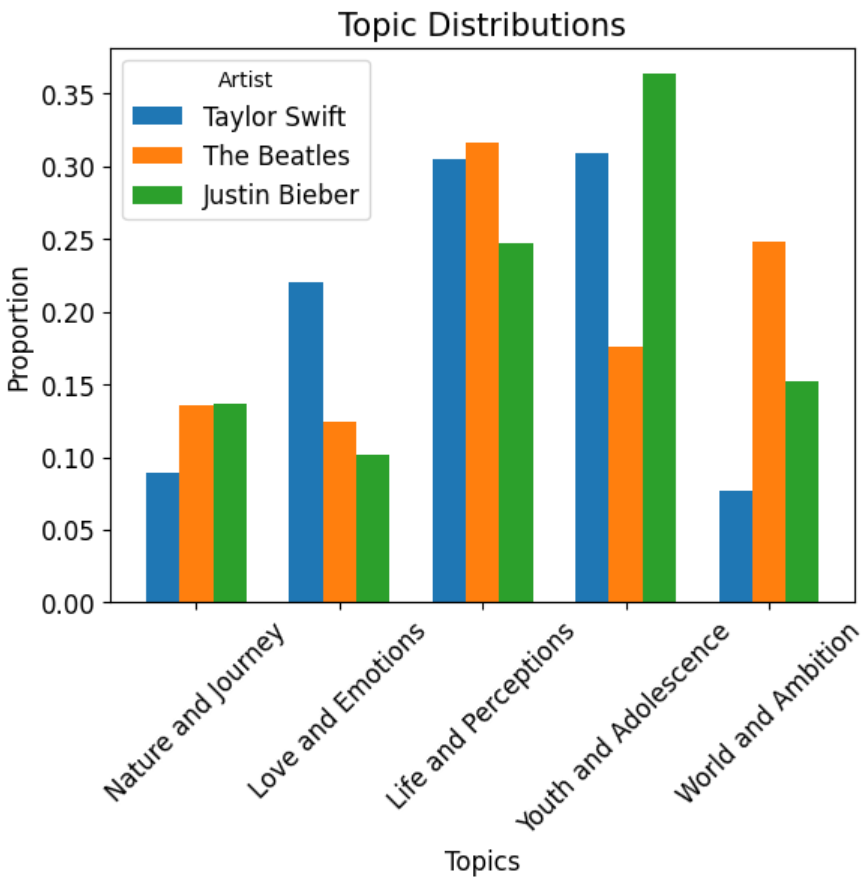
\includegraphics[width=0.5\textwidth]{artists.png}
    \caption{Topic Distribution for Taylor Swift, The Beatles and Justin Bieber}
\label{artists}
\end{figure}

\noindent Further, we analyzed the distribution of topics across different music genres. The result is shown in Figure~\ref{genres}. The major topics of Hip Hop are "Life and Perceptions" and "Youth and Adolescence". Country and Pop both have an remarkable emphasis on "Youth and Adolescence". Rock, Jazz and Old Pop, however, have a relatively more balanced representation across all themes, with slightly different preference over the topics: Rock considers more "World and Ambition", Jazz has more "Nature and Journey" content, and Old Pop sings more "Life and Perceptions".
\begin{figure}[H]
    \centering
    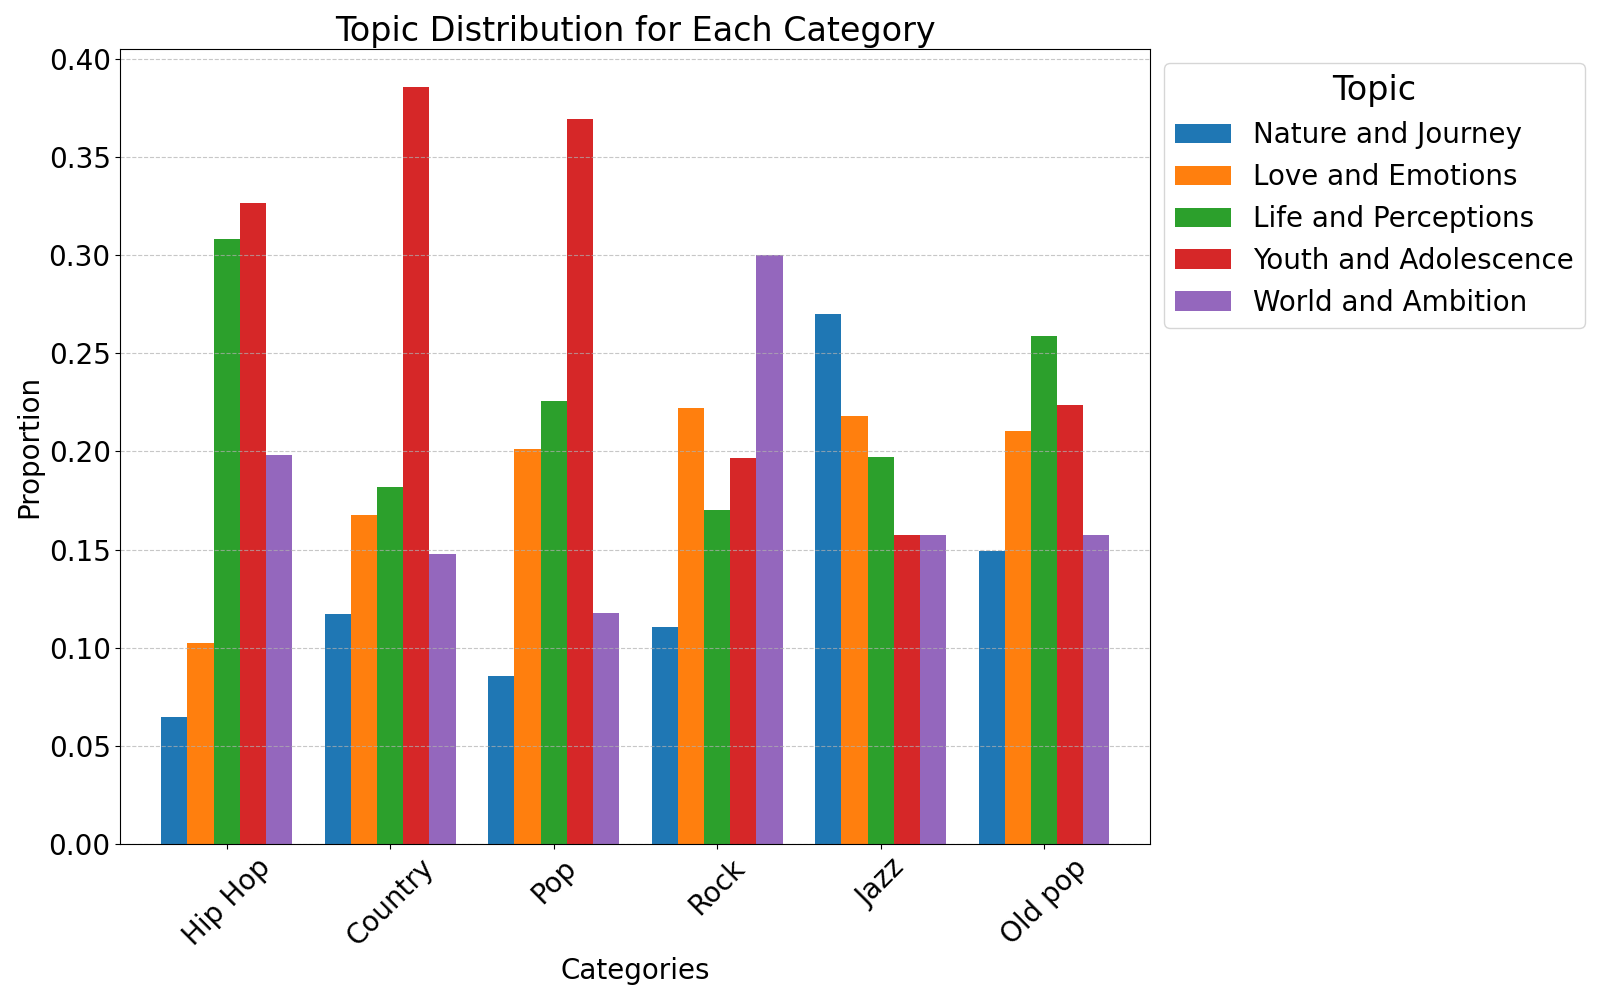
\includegraphics[width=0.8\textwidth]{genres.png}
    \caption{Topic Distribution for Different Music Genres}
    \label{genres}    
\end{figure}

\section{Discussion}

\noindent The results of the LDA model reveal distinct themes in the song lyrics, reflecting common topics such as love, life, relationships, and experiences. The identification of these themes helps in understanding the emotional and cultural significance of the lyrics. As we mentioned in Section~\ref{sec:introduction}, the reason we use LDA, not Dictionary Learning, for lyrics processing is that it excels in extracting thematic content from text, unlike Dictionary Learning, which is better suited for data requiring sparse representation and reconstruction.\\


\section{Conclusion}

\noindent The LDA model successfully categorized the lyrics into meaningful topics. Each topic represents a distinct theme commonly found in song lyrics, such as love, life, relationships, and experiences. This analysis provides a deeper understanding of the thematic content in song lyrics and can be used for further analysis or applications in music recommendation systems.

\section{Future Work}

For future work, more advanced models like bidirectional encoder representations from transformers (BERT)~\cite{devlin2018bert} can be used to capture deeper contextual relationships in the lyrics, and log-linear models can be used to reduce computational complexity~\cite{mikolov2013efficient}. Additionally, increasing the number of topics or fine-tuning the preprocessing steps might yield even more precise categorizations. Future studies could also explore the temporal changes in song lyrics topics over the years or across different cultural contexts.

\printbibliography

\newpage
\section*{Appendix}
\begin{lstlisting}[language=Python]
from lyricsgenius import Genius
import pandas as pd
import numpy as np
from langdetect import detect, LangDetectException
import nltk 
from nltk.corpus import stopwords, words
from nltk.tokenize import word_tokenize
from sklearn.feature_extraction.text import TfidfVectorizer, CountVectorizer
from sklearn.decomposition import LatentDirichletAllocation
import time

token = "<your-token>"
genius = Genius(token)


# Download necessary NLTK data
nltk.download('punkt')
nltk.download('stopwords')

# Dictionary of categories and representative singers
categories = {
    "Hip Hop": ["Kanye West", "Drake", "Kendrick Lamar", "Nicki Minaj", "Cardi B"],
    "Country": ["Johnny Cash", "Dolly Parton", "Luke Bryan", "Carrie Underwood", "Blake Shelton"],
    "Pop": ["Taylor Swift", "Ariana Grande", "Justin Bieber", "Katy Perry", "Lady Gaga"],
    "Rock": ["Queen", "Led Zeppelin", "The Beatles", "AC/DC", "Pink Floyd"],
    "Jazz": ["Louis Armstrong", "Ella Fitzgerald", "Duke Ellington", "Billie Holiday", "Miles Davis"],
    "Old pop": ["Michael Jackson", "John Lennon", "Bob Marley", "Stevie Wonder", "U2"]
}

# Function to get songs data for an artist
def get_songs_data(artist_name, max_songs):
    artist = genius.search_artist(artist_name, max_songs=max_songs)
    return [(song.title, song.lyrics) for song in artist.songs]

# Collect lyrics data
all_songs_data = []
for category, artists in categories.items():
    for artist in artists:
        try:
            songs_data = get_songs_data(artist, 20)  # Fetch 20 songs for each artist
            english_songs_data = [song for song in songs_data if detect(song[1]) == 'en']
            all_songs_data.extend([(category, artist, title, lyrics) for title, lyrics in english_songs_data])
            print(f"Collected songs for artist: {artist} in category: {category}")
            time.sleep(2)  # To avoid rate limiting
        except Exception as e:
            print(f"Failed to collect songs for artist {artist}: {e}")

# Create a DataFrame
df = pd.DataFrame(all_songs_data, columns=["category", "artist", "title", "lyrics"])

# Save DataFrame to CSV
df.to_csv("variety_lyrics_data.csv", index=False)


# Load lyrics data
df = pd.read_csv("variety_lyrics_data.csv")
# df = pd.read_csv("lyrics_data.csv")

# Function to filter and preprocess lyrics
stop_words = set(stopwords.words('english'))
stop_words.update(["mo", "pa", "bam","di","perry","bien","ta","say","said","make","come","got","let","chorus","yes","gon", "wo", "oh", "ca", "ai", "yeah", "travis", "wan", "hey", "ooh", "la", "da", "na", "eh", "ah", "whoa", "uh", "woo", "wow", "ohh", "oohh", "laa", "daa", "naa", "ehh", "ahh", "whoaa", "uhh", "wooo", "woww", "ohhh", "oohhh", "laaa", "daaa", "naaa", "ehhh", "ahhh", "whoaaa", "uhhh", "woooo", "wowww", "ohhhh", "oohhhh", "laaaa", "daaaa", "naaaa", "ehhhh", "ahhhh", "whoaaaa", "uhhhh", "wooooo", "wowwww", "ohhhhh", "oohhhhh", "laaaaa", "daaaaa", "naaaaa", "ehhhh", "ahhhh", "whoaaaaa", "uhhhhh", "woooooo", "wowwwww", "ohhhhhh", "oohhhhhh", "laaaaaa", "daaaaaa", "naaaaaa", "ehhhhh", "ahhhhh", "whoaaaaaa", "uhhhhhh", "wooooooo", "wowwwwww", "ohhhhhhh", "oohhhhhhh", "laaaaaaa", "daaaaaaa", "naaaaaaa", "ehhhhhh", "ahhhhhh", "whoaaaaaaa", "uhhhhhhh", "woooooooo", "wowwwwwww", "ohhhhhhhh", "oohhhhhhhh", "laaaaaaaa", "daaaaaaaa", "naaaaaaaa", "ehhhhhhh", "ahhhhhhh", "whoaaaaaaaa", "uhhhhhhhh", "wooooooooo", "wowwwwwwww", "ohhhhhhhhh", "oohhhhhhhhh", "laaaaaaaaa", "daaaaaaaaa", "naaaaaaaaa", "ehhhhhhhh", "ahhhhhhhh", "whoaaaaaaaaa", "uhhhhhhhhh", "woooooooooo", "wowwwwwwwww", "ohhhhhhhhhh", "oohhhhhhhhhh", "laaaaaaaaaa", "daaaaaaaaaa", "naaaaaaaaaa", "ehhhhhhhhh"])
valid_words = set(words.words())

def preprocess_lyrics(lyrics):
    tokens = word_tokenize(lyrics.lower())
    filtered_tokens = [word for word in tokens if word.isalnum() and word not in stop_words and word in valid_words]
    english_lyrics = []
    for word in filtered_tokens:
        if word.isalpha():  # Check if the word is an English alphabetic word
            english_lyrics.append(word)
    return ' '.join(english_lyrics)

df['processed_lyrics'] = df['lyrics'].apply(preprocess_lyrics)

# Vectorize the lyrics
vectorizer = TfidfVectorizer(max_features=1000, max_df=0.5, min_df=0.1, stop_words='english')
dtm = vectorizer.fit_transform(df['processed_lyrics'])

# Perform LDA
lda = LatentDirichletAllocation(n_components=5, random_state=1)
lda.fit(dtm)

# Display the topics
def display_topics(model, feature_names, no_top_words):
    for topic_idx, topic in enumerate(model.components_):
        print("Topic %d:" % (topic_idx))
        print(" ".join([feature_names[i] for i in topic.argsort()[:-no_top_words - 1:-1]]))

no_top_words = 10
tf_feature_names = vectorizer.get_feature_names_out()
display_topics(lda, tf_feature_names, no_top_words)

# Function to display the top words and their scores for each topic
def display_topics_with_scores(model, feature_names, no_top_words):
    for topic_idx, topic in enumerate(model.components_):
        print(f"Topic {topic_idx}:")
        top_words_scores = [(feature_names[i], topic[i]) for i in topic.argsort()[:-no_top_words - 1:-1]]
        for word, score in top_words_scores:
            print(f"{word}: {score:.4f}")
        print("\n")

# Number of top words to display
no_top_words = 5

# Assuming your LDA model and vectorizer are already fitted and named `lda` and `vectorizer`, respectively
# Get feature names (words) from the vectorizer
feature_names = vectorizer.get_feature_names_out()

# Display the topics and their scores
display_topics_with_scores(lda, feature_names, no_top_words)

# Get the topic distribution for each song
topic_values = lda.transform(dtm)

# Rename the topics based on the summaries
topic_names = {
    0: "Journey/Experience",
    1: "Love/Desire",
    2: "Life/Contemplation",
    3: "Relationships/Belief",
    4: "Wealth/World"
}

# Create a DataFrame to display the topic values for each song
topic_values_df = pd.DataFrame(topic_values, columns=[topic_names[i] for i in range(lda.n_components)])
result_df = pd.concat([df[['artist', 'title']], topic_values_df], axis=1)

# Display the topic values for all songs
print(result_df.head())

# Save the topic values to a CSV file
result_df.to_csv("topic_distribution.csv", index=False)

import matplotlib.pyplot as plt
topic_names = ["Nature and Journey", "Love and Emotions", "Life and Perceptions", "Youth and Adolescence", "World and Ambition"]

def get_topic_distribution(artist_name):
    # Filter the artist's songs
    artist_songs = df[df['artist'] == artist_name]
    artist_songs['processed_lyrics'] = artist_songs['lyrics'].apply(preprocess_lyrics)
    
    # Vectorize the artist's lyrics using the same vectorizer
    artist_dtm = vectorizer.transform(artist_songs['processed_lyrics'])
    
    # Use the trained LDA model to get topic distributions
    artist_topic_distributions = lda.transform(artist_dtm)
    
    # Convert topic distributions to a DataFrame
    artist_topic_vectors_df = pd.DataFrame(artist_topic_distributions, columns=[f"Topic {i}" for i in range(num_topics)])
    
    # Calculate the mean topic distribution
    artist_mean_topic_distribution = artist_topic_vectors_df.mean()
    
    return artist_mean_topic_distribution

# Get topic distributions for Taylor Swift and The Beatles
taylor_topic_distribution = get_topic_distribution('Taylor Swift')
beatles_topic_distribution = get_topic_distribution('The Beatles')
justin_topic_distribution = get_topic_distribution('Justin Bieber')

# Combine the topic distributions into one DataFrame
combined_df = pd.DataFrame({
    'Taylor Swift': taylor_topic_distribution,
    'The Beatles': beatles_topic_distribution,
    'Justin Bieber': justin_topic_distribution
})

# Plot the combined topic distributions
plt.figure(figsize=(16, 20))
combined_df.plot(kind='bar', width=0.7)
plt.title("Topic Distributions", fontsize=15)
plt.xlabel("Topics", fontsize=12)
plt.ylabel("Proportion", fontsize=12)
plt.xticks(ticks=range(num_topics), labels=topic_names, rotation=45, fontsize=12)
plt.yticks(fontsize=12)
plt.legend(title="Artist", fontsize=12)
plt.show()

import matplotlib.pyplot as plt

# Define summarized topic names
topic_names = ["Nature and Journey", "Love and Emotions", "Life and Perceptions", "Youth and Adolescence", "World and Ambition"]

def get_category_topic_distribution(category_name):
    # Filter the category's songs
    category_songs = df[df['category'] == category_name]
    category_songs['processed_lyrics'] = category_songs['lyrics'].apply(preprocess_lyrics)
    
    # Vectorize the category's lyrics using the same vectorizer
    category_dtm = vectorizer.transform(category_songs['processed_lyrics'])
    
    # Use the trained LDA model to get topic distributions
    category_topic_distributions = lda.transform(category_dtm)
    
    # Convert topic distributions to a DataFrame
    category_topic_vectors_df = pd.DataFrame(category_topic_distributions, columns=[f"Topic {i}" for i in range(num_topics)])
    
    # Calculate the mean topic distribution
    category_mean_topic_distribution = category_topic_vectors_df.mean()
    
    return category_mean_topic_distribution

# List of categories
categories = df['category'].unique()

# Get topic distributions for each category
category_distributions = {category: get_category_topic_distribution(category) for category in categories}

# Combine the topic distributions into one DataFrame
combined_category_df = pd.DataFrame(category_distributions).T
combined_category_df.columns = topic_names

# Plot the combined topic distributions
plt.figure(figsize=(14, 8))
combined_category_df.plot(kind='bar', width=0.8, figsize=(16, 10))
plt.title("Topic Distribution for Each Category", fontsize=24)
plt.xlabel("Categories", fontsize=20)
plt.ylabel("Proportion", fontsize=20)
plt.xticks(rotation=45, fontsize=20)
plt.yticks(fontsize=20)
plt.legend(title="Topic", fontsize=20, title_fontsize=24, loc='upper left', bbox_to_anchor=(1, 1))
plt.grid(axis='y', linestyle='--', alpha=0.7)
plt.tight_layout()
plt.savefig('genres.png')
plt.show()

\end{lstlisting}





\end{document}
